\documentclass[10pt, a4paper]{article}

\usepackage[utf8]{inputenc}
\usepackage[T1, T2A]{fontenc}
\usepackage[]{cmsrb}
\usepackage[margin=0.4in]{geometry}
\usepackage[serbian]{babel}
\usepackage{ifthen}

%\setcounter{errorcontextlines}{999}
%\documentclass{article}
%\usepackage[T1]{fontenc}
%\usepackage[latin1]{inputenc}
\usepackage{soulutf8}
\usepackage{color}
\makeatletter
\newcommand*{\whiten}[1]{\llap{\textcolor{white}{{\the\SOUL@token}}\hspace{#1pt}}}
\DeclareRobustCommand*\myul{%
    \def\SOUL@everyspace{\underline{\space}\kern\z@}%
    \def\SOUL@everytoken{%
     \setbox0=\hbox{\the\SOUL@token}%
     \ifdim\dp0>\z@
        \raisebox{\dp0}{\underline{\phantom{\the\SOUL@token}}}%
        \whiten{1}\whiten{0}%
        \whiten{-1}\whiten{-2}%
        \llap{\the\SOUL@token}%
     \else
        \underline{\the\SOUL@token}%
     \fi}%
\SOUL@}
\makeatother
 

\usepackage[Symbolsmallscale]{upgreek}
\usepackage{fancybox, graphicx}
\usepackage{enumitem}
\newcommand{\spacer}{\hspace*{5mm}}

\usepackage{amsmath, amsfonts}
\usepackage{icomma}
\usepackage{multirow}
\usepackage[table,xcdraw]{xcolor}

\pagestyle{empty} 

\usepackage{newtxmath}

\usepackage{tikz}
\newcommand*\circled[1]{\tikz[baseline=(char.base)]{
            \node[shape=circle,draw,inner sep=1pt] (char) {#1};}}

\let\sigma\upsigma
\let\omega\upomega

\frenchspacing

\newcommand{\unit}[1]{{\rm\,#1}}
\newcommand{\jj}{{\rm j}}
\newcommand{\ee}{{\rm e}}
\newcommand{\de}{{\rm d}}
\newcommand{\uu}{{\rm u}}
\newcommand{\DD}{{\rm D}}

\newcommand{\faz}[1]{\ensuremath{\underline{#1}}}

\newcommand{\ID}[0]{0}

\renewcommand{\infty}{
\includegraphics[scale=1]{inf.pdf}}


\usepackage{tabularx} % in the preamble

\newboolean{opcijeZaPolaganje} 
% Postaviti datum ispita koji se koristi u ostatku fajla
% prema tom datumu imenovati i glavni .tex fajl!
%
% Taj fajl treba da se zove si1oe_XXX_YY-ZZ.tex , gde je
%   - XXX sifra ispita malim slovima {jan, feb, jun, jul, aug, okt}
%   - YY-ZZ skolska godina, u formatu 2023/2024 |-->  23-24
% Isto ime promeniti i u settings.json !
%
\newcommand{\datumIspita}{xx.xx.xxxx. г}

% Setovati da li se nude opcije za polaganje ispita {true/false}
\setboolean{opcijeZaPolaganje}{true}  


\newcommand{\printheader}
{
\begin{flushright}
    \hfill
    \datumIspita
\end{flushright}
\vspace*{-35pt}
\begin{center}
    Електротехнички факултет 
    Универзитета у Београду --- Катедра за Електронику \\
    \textbf{ИСПИТ ИЗ ОСНОВА ЕЛЕКТРОНИКЕ \\ Одсек за софтверско инжењерство}
\end{center}
}

\begin{document}

\printheader

\vspace*{-1mm}
\noindent
\doublebox{%
\begin{minipage}[c]{\textwidth} \small
\textbf{Напомене.} 
Израда одабране опције траjе 180 минута. Није дозвољено
напуштање сале 60 минута од почетка израде задатака. Дозвољено jе читко
писање
графитном оловком. Дозвољена jе употреба овог формулара и једне испитне
вежбанке. Дозвољена jе и употреба непрограмабилних
калкулатора.
Градиво jе подељено по колоквиjумима. Сваки колоквиjум састављен jе из два
питања и jедног задатка. Бодовање питања и задатака означено jе
угластим
заградама иза одговараjуће ознаке тачке.
Задатке решавати \textbf{искључиво} у вежбанци, полазећи од \textbf{прве} стране.
Коначне одговоре на питања уписати у предвиђена поља, или заокружити
понуђене одговоре. Бодују се \myul{\textbf{само}} тачно одговорена питања.
Вежбанка се може користити и за припрему одговора на питања која захтевају извођење,
полазећи од \textbf{последње} стране вежбанке (таj део рада се не прегледа), а
коначан поступак треба да се налази на белинама формулара, и служи да се
провери оригиналност решења (\textit{одговори без извођења неће бити признати}).
У питањима у коjима се бира понуђени одговор, тачан одговор доноси
назначене поене, одговор „\textit{Не знам}“ или празно носи 0 поена, а погрешан
одговор носи $-1$ поен. \\[0.5mm]
Питања и задаци ће бити прегледани само уколико се налазе на \textbf{предвиђеним}
местима.
\end{minipage}}

\vspace{2mm}
\noindent
\textbf{Попунити податке о студенту 
\myul{хемијском оловком}. Исте податке 
исписати и на омоту вежбанке.
} 
%
\begin{center}
\vspace*{0mm} 
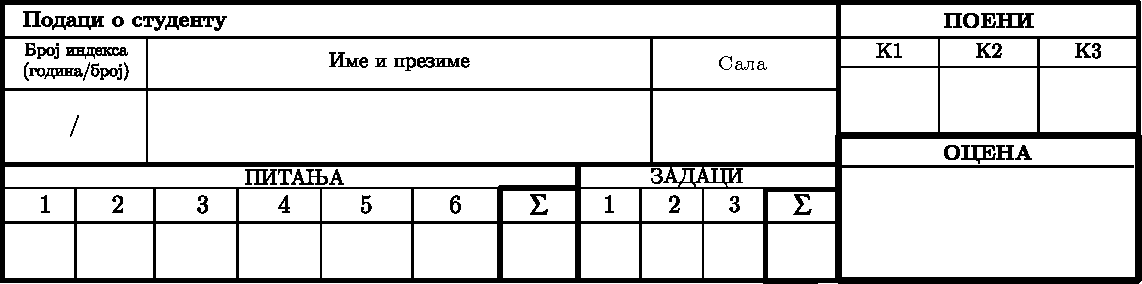
\includegraphics[scale=1]{si1oe_tablica_ispit.pdf}
\end{center}

\ifthenelse{\boolean{opcijeZaPolaganje}}{
    \noindent
    \textbf{\myul{Обавезно} заокружити опцију за полагање испита:}
    \hfill
    (\textit{i}) Само К3
    (\textit{ii}) К1 и К3
    (\textit{iii}) К2 и К3
    (\textit{iv}) K1, К2 и К3 \\[1mm]
    \textbf{Одабрану опцију назначити \myul{и на корици вежбанке}.} \\
}{
    \begin{center}
        ИНТЕГРАЛНИ ИСПИТ \\
    \end{center}
}
\noindent
\textbf{\large Први колоквијум}. \hrulefill \\

\vspace*{0mm}
\noindent
\textbf{Задатак}. \\[0.5mm]
\renewcommand{\ID}{1}\noindent
\textbf{\ID.}

\noindent\textbf{Питања.} \\[.5mm]
%
\renewcommand{\ID}{1}\noindent
\textbf{\ID.}


\renewcommand{\ID}{2}\noindent
\textbf{\ID.} 



\newpage 
\noindent
\textbf{\large Други колоквијум}. \hrulefill \\
\noindent
\textbf{Задатак}. \\[0.5mm]
\renewcommand{\ID}{2}\noindent
\textbf{\ID.} 

\noindent\textbf{Питања.} \\[1mm]
%
\renewcommand{\ID}{3}\noindent
\textbf{\ID.} 


\renewcommand{\ID}{4}\noindent
\textbf{\ID.} 


\newpage

\vspace{2mm}
\noindent
\textbf{Попунити податке о студенту 
\myul{хемијском оловком}. Исте податке 
исписати и на омоту вежбанке.
} 
%
\begin{center}
\vspace*{0mm} 
\includegraphics[scale=1]{SIS-tablica.pdf}
\end{center}

\noindent
\textbf{\large Трећи колоквијум}. \hrulefill \\

\vspace*{2mm}
\noindent
\textbf{Задатак}. \\[0.5mm]
\renewcommand{\ID}{3}\noindent
\textbf{\ID.} 


\vspace{5mm}
\noindent\textbf{Питања.} 

\renewcommand{\ID}{5}\noindent
\textbf{\ID.}


\vspace*{2mm}
\renewcommand{\ID}{6}\noindent
\textbf{\ID.}



%\end{document}

\newpage

\printheader
\begin{center}    
    \large \textbf{Одговори на питања 
    и решења задатака}    
\end{center}


\noindent
\textbf{\large Питања}. \\[0.5mm]

\renewcommand{\ID}{1}\noindent
\textbf{\ID.}


\vspace*{5mm}
\renewcommand{\ID}{2}\noindent
\textbf{\ID.}
\\[10mm]
\renewcommand{\ID}{3}\noindent
\textbf{\ID.}

\\[10mm]
\renewcommand{\ID}{4}\noindent
\textbf{\ID.}

\\[10mm]
\renewcommand{\ID}{5}\noindent
\textbf{\ID.}

\\[10mm]
\renewcommand{\ID}{6}\noindent
\textbf{\ID.}

\vspace*{5mm}

\noindent
\textbf{\large Задаци}. \\[0.5mm]

\renewcommand{\ID}{1}\noindent 
\textbf{\ID.} 
\\[10mm]
\renewcommand{\ID}{2}\noindent 
\textbf{\ID.}
\\[10mm]
\renewcommand{\ID}{3}\noindent
\textbf{\ID.}


\end{document}
